\section{Variance Reduction}
\begin{frame}{}
    \LARGE Reinforcement Learning: \textbf{Variance Reduction}
\end{frame}

\begin{frame}{Variance Reduction}
\begin{itemize}
    \item However, there is a problem.
    \item This approach suffers from high variance because credit assignment is difficult.
    \item Can we help the estimator?
    \pause
    \item \textbf{First idea:} Increase the probability of an action only by the cumulative future reward from that state:
    $$\nabla_\theta \mathcal{J}(\theta) \approx \sum_{t \geq 0} \left( \sum_{t' \geq t} r_{t'} \right ) \nabla_\theta \log \pi_\theta (a_t|s_t) $$
\end{itemize}
\end{frame}

\begin{frame}{Variance Reduction}
\begin{figure}
\centering
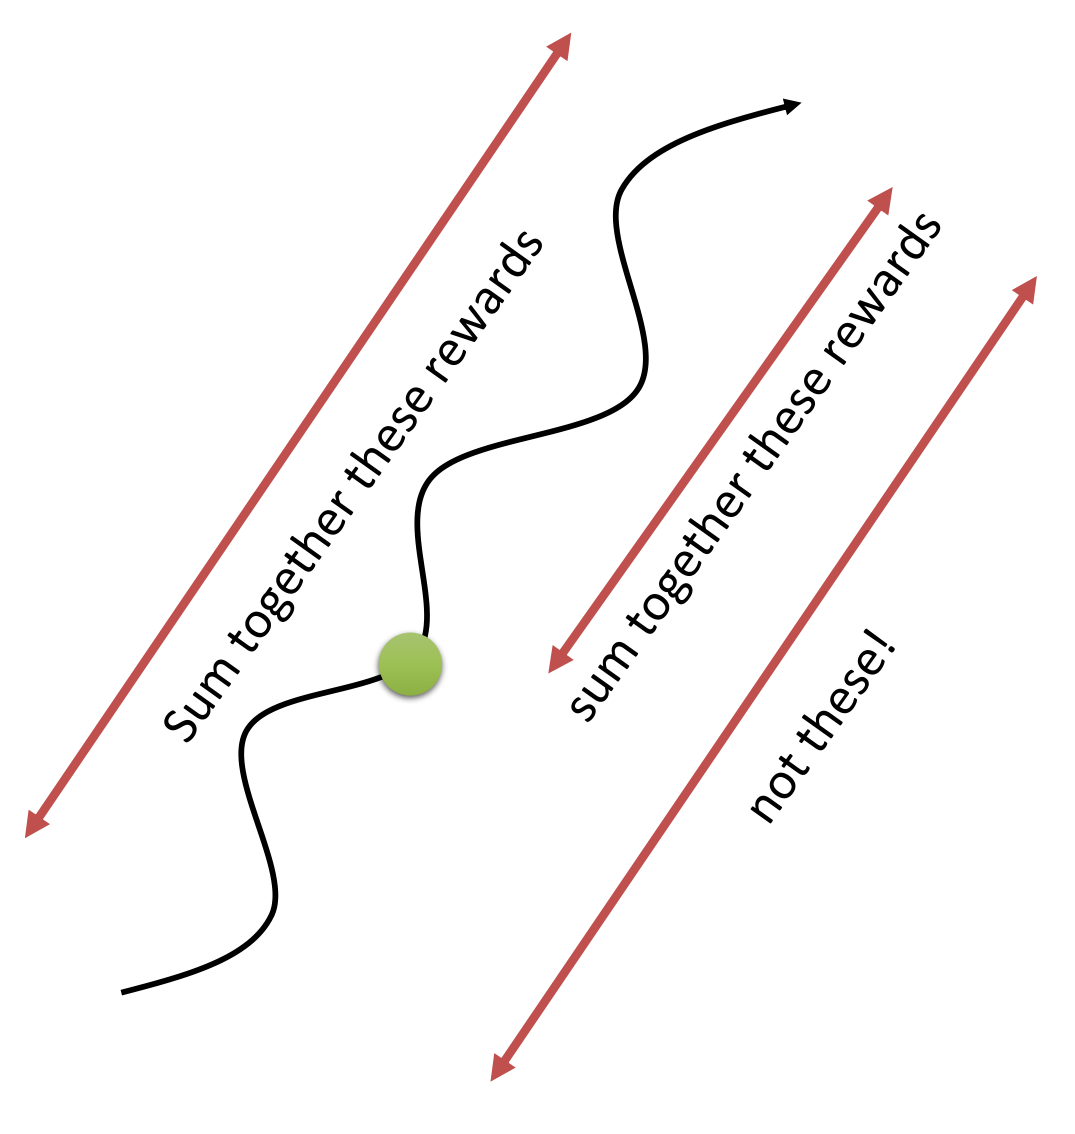
\includegraphics[width=0.9\textwidth,height=0.9\textheight,keepaspectratio]{images/policygrad+reinforce+actor/var_red_1.png}
\end{figure}
\end{frame}

\begin{frame}{Variance Reduction}
\begin{itemize}
    \item But this still doesn't completely solve the credit assignment problem.
    \item It can lead to bias due to delayed rewards.
    \pause
    \item \textbf{Second idea:} Use a discount factor $\gamma$ to reduce the effect of delayed rewards:
    $$\nabla_\theta \mathcal{J}(\theta) \approx \sum_{t \geq 0} \left( \sum_{t' \geq t} \gamma^{t'-t} r_{t'} \right ) \nabla_\theta \log \pi_\theta (a_t|s_t) $$
\end{itemize}
\end{frame}

\begin{frame}{Variance Reduction}
\begin{figure}
\centering
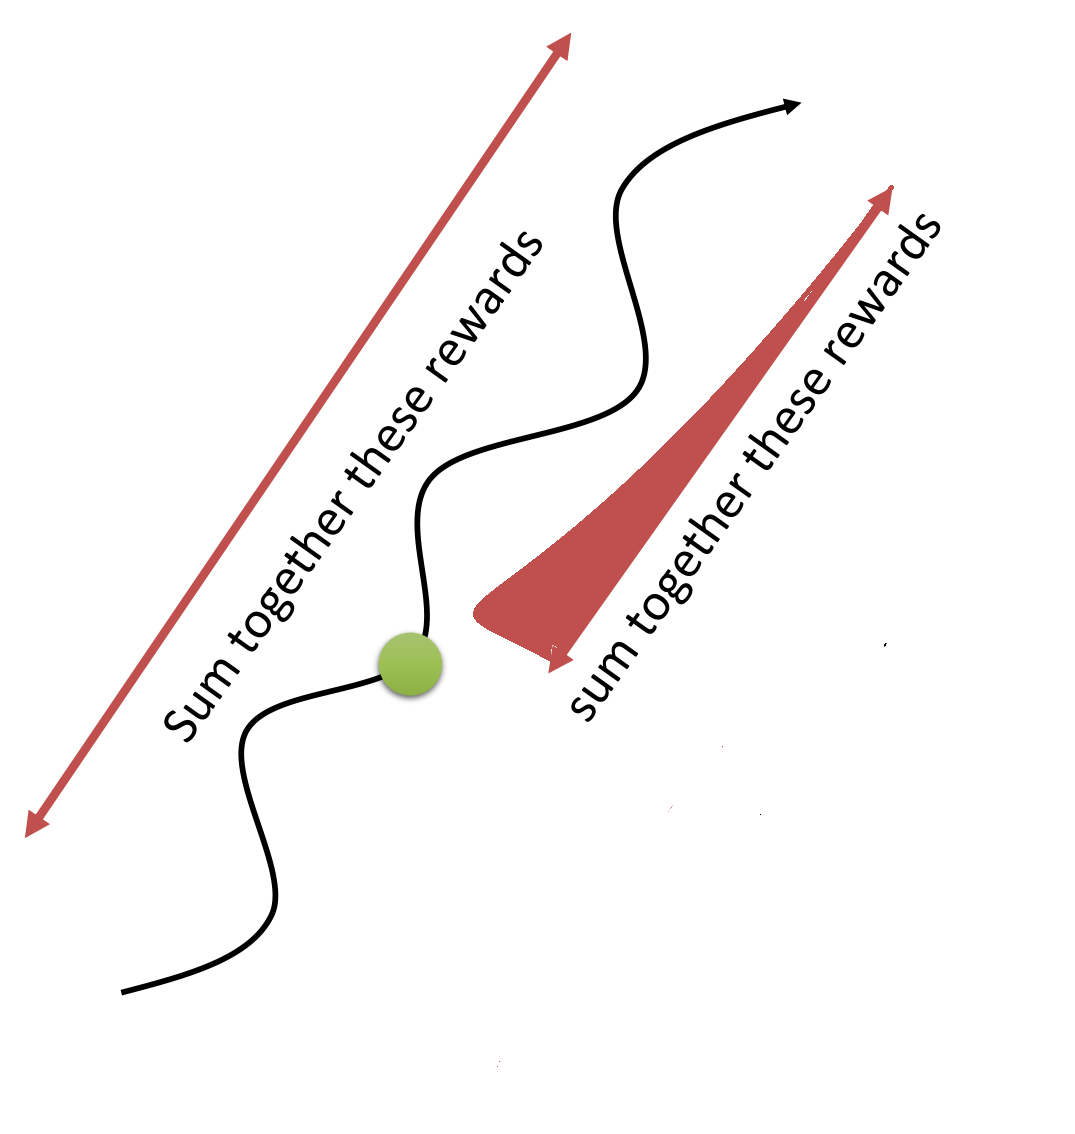
\includegraphics[width=0.9\textwidth,height=0.9\textheight,keepaspectratio]{images/policygrad+reinforce+actor/var_red_2.png}
\end{figure}
\end{frame}

\begin{frame}{Variance Reduction - Baselines}
\begin{itemize}
    \item \textbf{Problem:} The raw value of a trajectory isn’t necessarily meaningful. For example, if all rewards are positive, you keep increasing the probabilities of actions.
    \pause
    \item \textbf{What is important then?} Whether a reward is better or worse than what you expect to get.
    \pause
    \item \textbf{Idea:} Introduce a baseline function dependent on the state:
    $$\nabla_\theta \mathcal{J}(\theta) \approx \sum_{t \geq 0} \left( \sum_{t' \geq t} \gamma^{t'-t} r_{t'}  - b(s_t)\right ) \nabla_\theta \log \pi_\theta (a_t|s_t) $$
    \pause
    \item A simple baseline: the moving average of rewards experienced so far from all trajectories.
\end{itemize}
\end{frame}

\begin{frame}{How to Choose the Baseline?}
\begin{itemize}
    \item Can we choose a better baseline?
    \item Essentially, we want to increase the probability of an action from a state if this action was better than the \textbf{expected value} from that state.
    \pause
    \item What does this remind you of?
    \pause
    \item \textbf{Answer:} Q-function and value function!
\end{itemize}
\end{frame}

\begin{frame}{How to Choose the Baseline?}
\begin{itemize}
    \item Intuitively, we are happy with an action $a_t$ in a state $s_t$ if $Q^{\pi}(s_t, a_t) - V^{\pi}(s_t)$ is large. In contrast, we are unhappy if it is small.
    \pause
    \item The term $Q^{\pi}(s_t, a_t) - V^{\pi}(s_t)$ is called the \textbf{Advantage} and is denoted by $A^{\pi}(s_t, a_t)$.
    \pause
    \item Using this, we get the estimator:
    $$\nabla_\theta \mathcal{J}(\theta) \approx \sum_{t \geq 0} \left( Q^{\pi}(s_t, a_t) - V^{\pi}(s_t) \right ) \nabla_\theta \log \pi_\theta (a_t|s_t) $$
\end{itemize}
\end{frame}
